\documentclass{beamer}
%[utf8,compress,handout]
\usetheme{JuanLesPins}

%\usepackage[francais]{babel}
\usepackage[T1]{fontenc}
\usepackage[utf8]{inputenc}
\usepackage{hyperref}
\usepackage{graphicx}
\usepackage{multimedia}
\usepackage{float}
\usepackage{listings}
\usepackage{xcolor}
\usepackage{multicol}

\setbeamertemplate{footline}[frame number]

\titlegraphic{
	
\includegraphics[scale=0.05]{Logo-UJF.png}
	\hspace{5em}
\includegraphics[scale=0.05]{Logo_ENSIMAG.png}
  \hspace{5em}
\includegraphics[scale=0.05]{LIG.jpg}
}

\title{BDI multi-agent modelling of the population's decision making in a bushfire}
\author{Geoffrey DANET\\M2 MoSIG\\ supervised by Carole ADAM\\LIG - MAGMA team}
\date{$22^{nd}$ June 2016}

\expandafter\def\expandafter\insertshorttitle\expandafter{%
  \insertshorttitle\hfill%
}

\AtBeginSection[]
{
  \begin{frame}
    \frametitle{Table of Contents}
    \tableofcontents[currentsection]
  \end{frame}
}

\begin{document}

  \begin{frame}
    \titlepage
  \end{frame}

  \begin{frame}{Black Saturday}
    \begin{itemize}
      \item 7 February 2009,
      \item 173 dead et 414 injured,
      \item \begin{math}\sim\end{math} 450 000 ha burned.
      \item The expected behaviour is different from the reality,
    \end{itemize}
		SWIFT project:
    \newline
    $\rightarrow$ Make a serious game in order to raise the awareness of the emergency managers about the real population
    behaviour.
    \newline
    $\rightarrow$ Simulation must be as realistic as possible.
    \begin{figure}[h]
      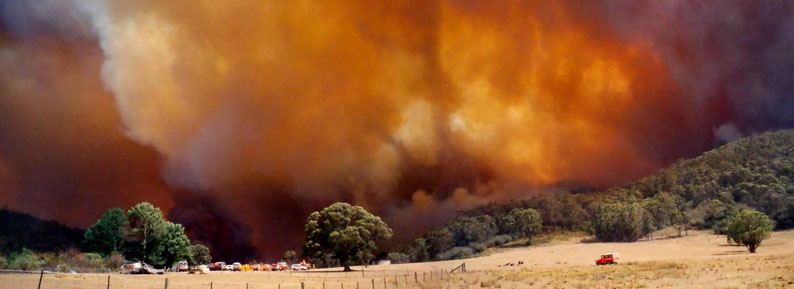
\includegraphics[scale=0.4]{canberra-2003-cropped.jpg}
    \end{figure}
  \end{frame}

  \begin{frame}{Computer simulation}
    \begin{block}{Why computer simulation ?}
      \begin{itemize}
        \item Repeatable,
        \item Controllable,
        \item Cheap,
        \item Safe.
      \end{itemize}
    \end{block}
		\begin{figure}[h]
			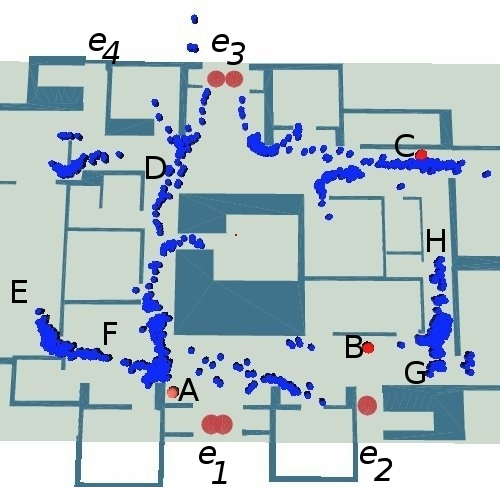
\includegraphics[scale=0.4]{eva2.jpg}
		\end{figure}
  \end{frame}

  \section{State Of the Art}

    \begin{frame}{State Of the Art}
      The existing simulations are focused on:
      \begin{itemize}
				\item Fire behaviour \cite{phoenix},
        \item The crowd behaviour during building and public area evacuation \cite{modeling2008,human2006,crowd2005},
				\begin{itemize}
					\item Basic and homogeneous behaviour,
					\item Lack of human factors (emotions, determination, ...),
					\item Ignores pre-evacuation.
				\end{itemize}
      \end{itemize}
			\vspace{2em}
			$\rightarrow$ Simulation based on a cognitive architecture.
    \end{frame}

		\begin{frame}{State Of the Art (2)}
			Simulations using a cognitive architecture exist but:
			\begin{itemize}
				\item Evacuation in public area \\ \qquad $\rightarrow$ behaviours are different in a personal house \\ \qquad ~~~ \cite{tsai2011},
				\item Focus on performance and scalability \\ \qquad $\rightarrow$ homogeneous behaviour without personality \\ \qquad ~~~ \cite{Cho2008}.
			\end{itemize}
			\vspace{2em}
			$\rightarrow$ Use a top-down approach \\ ~~~~(from the theory to the implementation).
		\end{frame}

    \begin{frame}{Proposal}
      \begin{itemize}
        \item Make a \textbf{realistic} simulation of Autralian population behaviour in bushfires.
        \item[$\rightarrow$] Require valid results,
        \item[$\rightarrow$] Use of cognitive architecture.
      \end{itemize}
      \begin{figure}[h]
        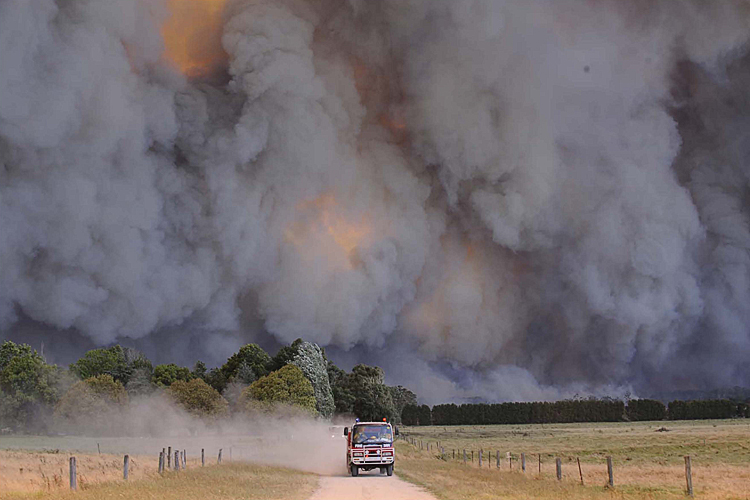
\includegraphics[scale=0.3]{PJ-1.jpg}
      \end{figure}
    \end{frame}

    \begin{frame}{Simulation Multi-Agent}
      \begin{block}{What is an agent?}
        Autonomous system which perceives and interacts with its environment.
      \end{block}
      \begin{itemize}
        \item Multiple agents coexist and interact.
				\item Different agent architectures of varying complexity.
      \end{itemize}
			\begin{figure}[h]
        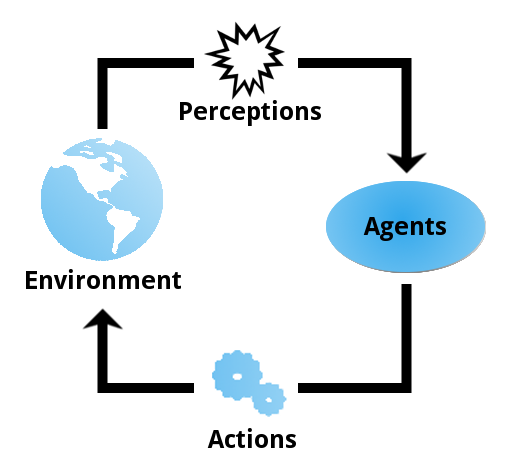
\includegraphics[scale=0.25]{mas_graph.png}
      \end{figure}
    \end{frame}

    \begin{frame}{Belief Desire Intention}
      \begin{block}{Beliefs}
        Information about the environment, itself or the other agents. It can be \textbf{incomplete} or \textbf{incorrect}.
      \end{block}
      \begin{block}{Desires}
        Motivations to do something. It can be \textbf{inconsistent} or \textbf{unrealistic}.
      \end{block}
      \begin{block}{Intentions}
				Leads to \textbf{action}. \\
				Selected from the \textbf{desires} and \textbf{beliefs} of the agent. It can have several associated \textbf{plans} allowing to achieve it.
      \end{block}
    \end{frame}

    \begin{frame}{Believe Desire Intention (2)}
      \vspace{-2em}
      \begin{figure}[h]
        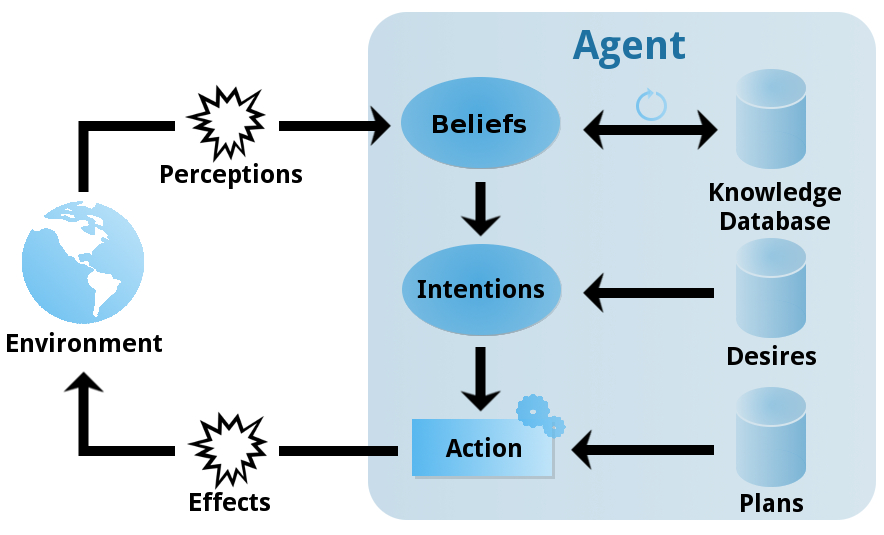
\includegraphics[scale=0.35]{bdi_graph.png}
      \end{figure}
    \end{frame}

  \section{Data and Tools}

    \begin{frame}{Witness Statement \cite{exell}}
      \begin{block}{Sue Exell}
        \begin{quote}
  				\textquotedblleft I $\textbf{looked}$ out the window and $\textbf{saw}$ some hazy smoke to the north-west ...\textquotedblright
        \end{quote}
      \end{block}
      \begin{itemize}
        \item[$\rightarrow$] Perception
      \end{itemize}
    \end{frame}

    \begin{frame}{Witness Statement \cite{exell}}
      \begin{block}{Sue Exell}
        \begin{quote}
  				\textquotedblleft ... Gary said that he $\textbf{thought}$ it was just dust but we went outside ...\textquotedblright
  			\end{quote}
      \end{block}
      \begin{itemize}
        \item[$\rightarrow$] Belief
      \end{itemize}
    \end{frame}


    \begin{frame}{Witness Statement \cite{exell}}
      \begin{block}{Sue Exell}
        \begin{quote}
  				\textquotedblleft ... and straight away we $\textbf{noticed}$ that we could $\textbf{smell}$ smoke ...\textquotedblright
  			\end{quote}
      \end{block}
      \begin{itemize}
        \item[$\rightarrow$] Perception
        \item[$\rightarrow$] New belief (updated)
      \end{itemize}
    \end{frame}

    \begin{frame}{Witness Statement \cite{exell}}
      \begin{block}{Sue Exell}
        \begin{quote}
          \textquotedblleft ... as soon as that happened, Gary agreed to \textbf{go and get the fire pump.} ...\textquotedblright
        \end{quote}
      \end{block}
      \begin{itemize}
        \item[$\rightarrow$] Intention : defend their property,
        \item[$\rightarrow$] First plan : Prepare the fire pump.
      \end{itemize}
    \end{frame}

    \begin{frame}{Tactics Decision Framework (TDF)}
      TDF is a tactical decision-making modelling tool based on the Prometheus methodology \cite{framework2015}.
      It provides:
      \begin{itemize}
        \item BDI Based paradigm,
        \item Structural modelling of missions, goals, scenarios, input/output, messaging and procedures.
      \end{itemize}
    \end{frame}

    \begin{frame}{Tactics Decision Framework (TDF) (2)}
      \begin{figure}[h]
        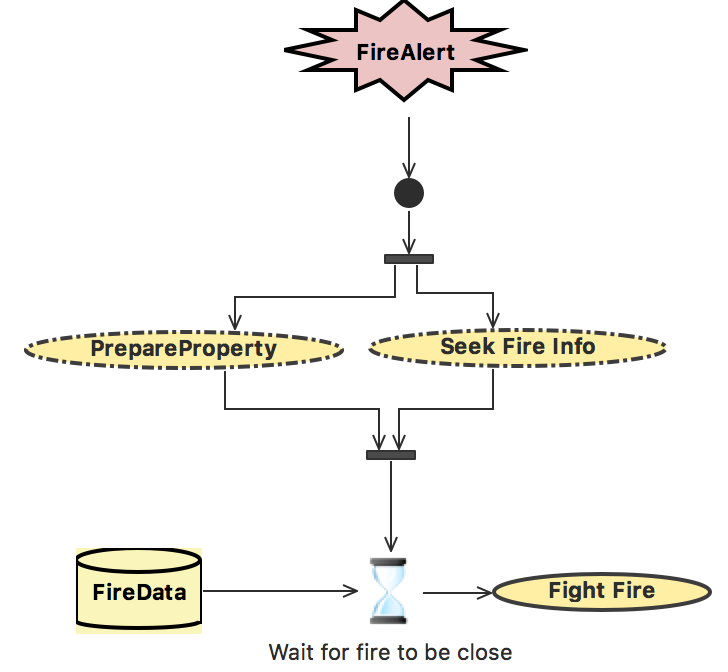
\includegraphics[scale=0.5]{plan.png}
        \caption{Plan diagram example}
      \end{figure}
    \end{frame}

    \begin{frame}{GAMA and GAML}
      \begin{itemize}
        \item Open source development platform
        \item GAML language
        \item BDI extension
      \end{itemize}
      \begin{block}{Perception exemple}
\textbf{perceive} \textbf{target}:fire \textbf{in}:perception\_radius \{\\
~~\textbf{add} self \textbf{to}: myself.known\_fires;\\
~~\textbf{ask} myself \{\\
~~~~\textbf{do} \textit{add\_belief}(fire);\\
~~\}\\
\}
      \end{block}
    \end{frame}

    \begin{frame}{Civilian's Profiles}
      A previous study by Alan Rhodes shows there are 6 existing profiles \cite{rhodes2014}:

      \begin{itemize}
        \item Can do defender: \textquotedblleft Just do it, just get on with it\textquotedblright
        \item Considered defender: \textquotedblleft You have to be prepared if you choose to live here\textquotedblright
        \item Livelihood defender: \textquotedblleft It's not just a house, it's our livelihood\textquotedblright
        \item Threat monitor: \textquotedblleft I'll leave when I need to - before it's really dangerous\textquotedblright
        \item Threat avoider: \textquotedblleft Life is more important than the house\textquotedblright
        \item Unaware reactor: \textquotedblleft I didn't expect a fire like that - I was shocked\textquotedblright
      \end{itemize}
    \end{frame}

  \section{Implementation}

    \begin{frame}{Implementation}
      BDI architecture based on a Finite State Machine (FSM) made in a previous study \cite{adam2015} and on the witness statements
      data \cite{witness}.
      \begin{itemize}
        \item Grid which represents the map,
        \item 200 \textquotedblleft Pedestrian\textquotedblright ~BDI agents (Australian citizens),
        \item 200 houses (one per Pedestrian agent),
        \item 2 shelters,
        \item Basic fire implementation (random propagation).
      \end{itemize}
    \end{frame}

    \begin{frame}{Graphical rendering}
      \vspace{-1em}
      \begin{figure}[h]
        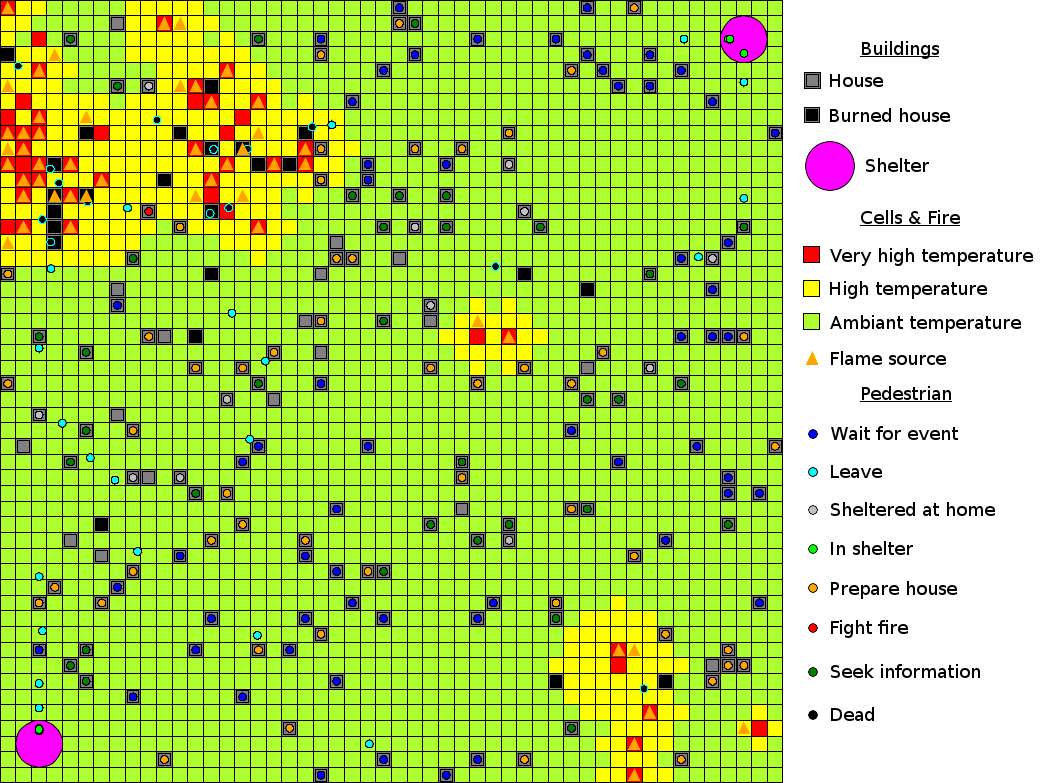
\includegraphics[scale=0.35]{simu-legends.png}
      \end{figure}
    \end{frame}

    \begin{frame}{Demo}
      \begin{figure}
        \vspace{-1.8em}
        \hspace*{-2em}
        \movie[width=12.3cm,height=7.2cm, poster, showcontrols]{vids-background.png}{simu-switf-gama.mp4}
      \end{figure}
    \end{frame}

  \section{Experiments and results}

    \begin{frame}{Experiments}
      \begin{itemize}
        \item 2 different parameters sets,
				\begin{itemize}
					\item Weak fire: low intensity and low propagation rate,
					\item Intense fire: high intensity and high propagation rate.
				\end{itemize}
        \item Each experiment includes 500 cycles and 10 simulation iterations,
        \item The results will be compared between them and with the statistics from the Victorian Bushfires Royal Commission \cite{stats2009},
      \end{itemize}
    \end{frame}

    \begin{frame}{Statistics}
      \begin{figure}[h]
        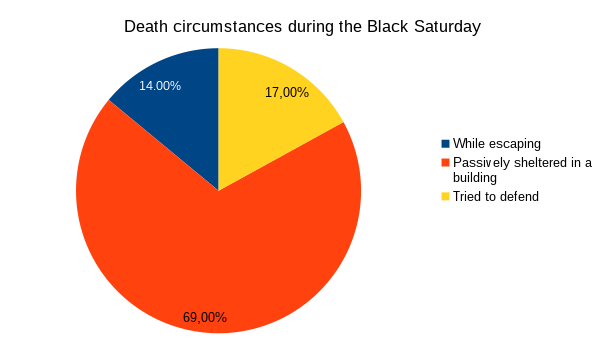
\includegraphics[scale=0.6]{stat.png}
      \end{figure}
    \end{frame}

    \begin{frame}{Result: death circumstances}
	      \begin{figure}[h]
	        \hspace*{-3em}
	        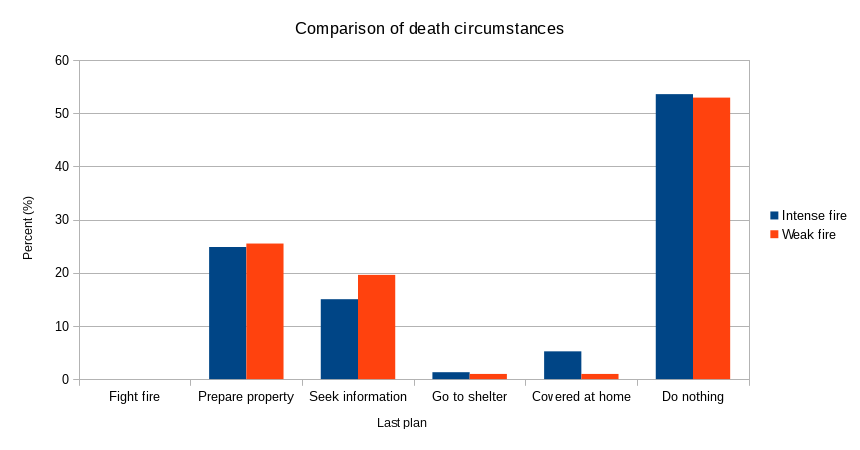
\includegraphics[scale=0.55]{last-plan-comparison.png}
	      \end{figure}
    \end{frame}

    \begin{frame}{Result: profiles}
      \begin{figure}[h]
        \hspace*{-3em}
        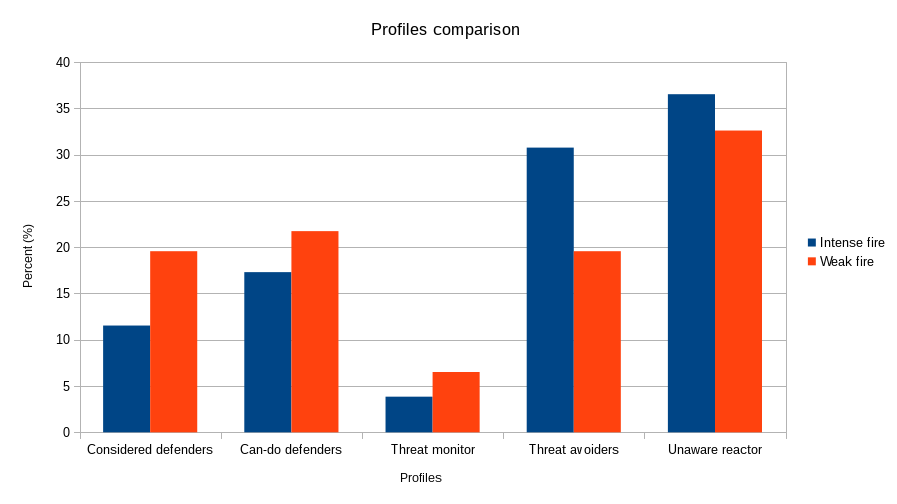
\includegraphics[scale=0.54]{profils-comparison.png}
      \end{figure}
    \end{frame}

  \section{Conclusion}

    \begin{frame}{Contribution}
      \begin{itemize}
        \item Followed a bottom-up methodology: \\ \qquad Interviews $\rightarrow$ TDF $\rightarrow$ GAMA,
        \item implemented a realistic BDI model,
				\item Studied model validity,
        \item Provided feedback on GAMA and TDF,
        \item Submitted paper to ISCRAM-med 2016 (under review).
      \end{itemize}
    \end{frame}

    \begin{frame}{Future Work}
      \begin{itemize}
        \item Compare BDI vs Finite State Machine (FSM),
        \item Improve the BDI implementation \\ \qquad (add emotions, social relationships...),
				\item Integrate a more realistic fire model \\ \qquad (SPARK \cite{Miller2015}),
				\item Take into account the topology (road, forest...)
        \item Subject of a PhD Thesis.
      \end{itemize}
    \end{frame}

		\begin{frame}{BDI multi-agent modelling of the population's decision making in a bushfire}
			\centering
			Questions are welcome.
			\begin{figure}[h]
        
\includegraphics[scale=0.2]{question.jpg}
      \end{figure}
		\end{frame}

  \footnotesize
  \bibliographystyle{apalike}
  \bibliography{biblio}

\end{document}
